% Options for packages loaded elsewhere
\PassOptionsToPackage{unicode}{hyperref}
\PassOptionsToPackage{hyphens}{url}
%
\documentclass[
  letterpaper,
]{book}

\usepackage{amsmath,amssymb}
\usepackage{iftex}
\ifPDFTeX
  \usepackage[T1]{fontenc}
  \usepackage[utf8]{inputenc}
  \usepackage{textcomp} % provide euro and other symbols
\else % if luatex or xetex
  \usepackage{unicode-math}
  \defaultfontfeatures{Scale=MatchLowercase}
  \defaultfontfeatures[\rmfamily]{Ligatures=TeX,Scale=1}
\fi
\usepackage{lmodern}
\ifPDFTeX\else  
    % xetex/luatex font selection
\fi
% Use upquote if available, for straight quotes in verbatim environments
\IfFileExists{upquote.sty}{\usepackage{upquote}}{}
\IfFileExists{microtype.sty}{% use microtype if available
  \usepackage[]{microtype}
  \UseMicrotypeSet[protrusion]{basicmath} % disable protrusion for tt fonts
}{}
\makeatletter
\@ifundefined{KOMAClassName}{% if non-KOMA class
  \IfFileExists{parskip.sty}{%
    \usepackage{parskip}
  }{% else
    \setlength{\parindent}{0pt}
    \setlength{\parskip}{6pt plus 2pt minus 1pt}}
}{% if KOMA class
  \KOMAoptions{parskip=half}}
\makeatother
\usepackage{xcolor}
\setlength{\emergencystretch}{3em} % prevent overfull lines
\setcounter{secnumdepth}{5}
% Make \paragraph and \subparagraph free-standing
\ifx\paragraph\undefined\else
  \let\oldparagraph\paragraph
  \renewcommand{\paragraph}[1]{\oldparagraph{#1}\mbox{}}
\fi
\ifx\subparagraph\undefined\else
  \let\oldsubparagraph\subparagraph
  \renewcommand{\subparagraph}[1]{\oldsubparagraph{#1}\mbox{}}
\fi


\providecommand{\tightlist}{%
  \setlength{\itemsep}{0pt}\setlength{\parskip}{0pt}}\usepackage{longtable,booktabs,array}
\usepackage{calc} % for calculating minipage widths
% Correct order of tables after \paragraph or \subparagraph
\usepackage{etoolbox}
\makeatletter
\patchcmd\longtable{\par}{\if@noskipsec\mbox{}\fi\par}{}{}
\makeatother
% Allow footnotes in longtable head/foot
\IfFileExists{footnotehyper.sty}{\usepackage{footnotehyper}}{\usepackage{footnote}}
\makesavenoteenv{longtable}
\usepackage{graphicx}
\makeatletter
\def\maxwidth{\ifdim\Gin@nat@width>\linewidth\linewidth\else\Gin@nat@width\fi}
\def\maxheight{\ifdim\Gin@nat@height>\textheight\textheight\else\Gin@nat@height\fi}
\makeatother
% Scale images if necessary, so that they will not overflow the page
% margins by default, and it is still possible to overwrite the defaults
% using explicit options in \includegraphics[width, height, ...]{}
\setkeys{Gin}{width=\maxwidth,height=\maxheight,keepaspectratio}
% Set default figure placement to htbp
\makeatletter
\def\fps@figure{htbp}
\makeatother

\makeatletter
\makeatother
\makeatletter
\@ifpackageloaded{bookmark}{}{\usepackage{bookmark}}
\makeatother
\makeatletter
\@ifpackageloaded{caption}{}{\usepackage{caption}}
\AtBeginDocument{%
\ifdefined\contentsname
  \renewcommand*\contentsname{Table of contents}
\else
  \newcommand\contentsname{Table of contents}
\fi
\ifdefined\listfigurename
  \renewcommand*\listfigurename{List of Figures}
\else
  \newcommand\listfigurename{List of Figures}
\fi
\ifdefined\listtablename
  \renewcommand*\listtablename{List of Tables}
\else
  \newcommand\listtablename{List of Tables}
\fi
\ifdefined\figurename
  \renewcommand*\figurename{Figure}
\else
  \newcommand\figurename{Figure}
\fi
\ifdefined\tablename
  \renewcommand*\tablename{Table}
\else
  \newcommand\tablename{Table}
\fi
}
\@ifpackageloaded{float}{}{\usepackage{float}}
\floatstyle{ruled}
\@ifundefined{c@chapter}{\newfloat{codelisting}{h}{lop}}{\newfloat{codelisting}{h}{lop}[chapter]}
\floatname{codelisting}{Listing}
\newcommand*\listoflistings{\listof{codelisting}{List of Listings}}
\makeatother
\makeatletter
\@ifpackageloaded{caption}{}{\usepackage{caption}}
\@ifpackageloaded{subcaption}{}{\usepackage{subcaption}}
\makeatother
\makeatletter
\@ifpackageloaded{tcolorbox}{}{\usepackage[skins,breakable]{tcolorbox}}
\makeatother
\makeatletter
\@ifundefined{shadecolor}{\definecolor{shadecolor}{rgb}{.97, .97, .97}}
\makeatother
\makeatletter
\makeatother
\makeatletter
\makeatother
\ifLuaTeX
  \usepackage{selnolig}  % disable illegal ligatures
\fi
\IfFileExists{bookmark.sty}{\usepackage{bookmark}}{\usepackage{hyperref}}
\IfFileExists{xurl.sty}{\usepackage{xurl}}{} % add URL line breaks if available
\urlstyle{same} % disable monospaced font for URLs
\hypersetup{
  pdftitle={Baroque AI: Publication Prototype},
  pdfauthor={Class participants},
  hidelinks,
  pdfcreator={LaTeX via pandoc}}

\title{Baroque AI: Publication Prototype}
\author{Class participants}
\date{2023-04-28}

\begin{document}
\frontmatter
\maketitle
\ifdefined\Shaded\renewenvironment{Shaded}{\begin{tcolorbox}[borderline west={3pt}{0pt}{shadecolor}, frame hidden, boxrule=0pt, interior hidden, breakable, sharp corners, enhanced]}{\end{tcolorbox}}\fi

\renewcommand*\contentsname{Table of contents}
{
\setcounter{tocdepth}{2}
\tableofcontents
}
\mainmatter
\bookmarksetup{startatroot}

\hypertarget{title}{%
\chapter{Title:}\label{title}}

Author: Ahmad Aroud

ORCID: https://orcid.org/0009-0000-3344-9566

Date: 28.04.2023

DOI: 10.5281/zenodo.7875479

Repository URL: https://github.com/AhmadAroud/catalogue-003

\hypertarget{based-on-baroque-ai-publication-prototype}{%
\section{Based on Baroque AI: Publication
Prototype}\label{based-on-baroque-ai-publication-prototype}}

\hypertarget{part-of-the-series-baroque-toc}{%
\section{Part of the series: Baroque
TOC}\label{part-of-the-series-baroque-toc}}

\href{https://nfdi4culture.github.io/class-ADA-CP-pipeline/}{Programme
instructions}

2023-03-17

This work is licensed under a Creative Commons Attribution-ShareAlike
4.0 International License.

Book cover: Reworking of
\href{https://en.wikipedia.org/wiki/File:Pendant_in_the_form_of_a_siren_MET_DT7173.jpg}{Baroque
pearl with enamelled gold mounts set with rubies}. Creative Commons CC0
1.0 Universal Public Domain Dedication. This file was donated to
Wikimedia Commons as part of a project by the Metropolitan Museum of
Art.

This work is licensed under a Creative Commons Attribution-ShareAlike
4.0 International License.

\bookmarksetup{startatroot}

\hypertarget{colophon}{%
\chapter{Colophon}\label{colophon}}

Fork title: AhmadAroud/catalogue-003

Author: Ahmad Aroud

ORCID: https://orcid.org/0009-0000-3344-9566

Date: 28.04.2023

DOI: 10.5281/zenodo.7875479

Repositor: https://github.com/AhmadAroud/catalogue-003

PUBLISHING FROM COLLECTIONS USES OF COMPUTATIONAL PUBLISHIGN AND
LINKEDOPEN DATA

Open Science Lab - TIB Hannnover

First published 2023-03-30

Copyright © The Authors 2023 Licensed as
https://creativecommons.org/licenses/by-sa/4.0/

DOI: https://doi.org/10.5281/zenodo.7701161

\bookmarksetup{startatroot}

\hypertarget{louvre}{%
\chapter{Louvre}\label{louvre}}

Source: https://de.wikipedia.org/wiki/Louvre

Der Ursprung der Sammlung geht auf das 14. Jahrhundert zurück. Der
Herzog Jean de Berry (1340--1415), ein Bruder Karls V., legte eine
Sammlung von Gemälden, Tapisserien und Buchmalereien an, von denen
einige noch in der heutigen Ausstellung zu sehen sind. Mona Lisa
(Leonardo da Vinci, 1503--1505)

Der eigentliche Begründer der Sammlung ist aber König Franz I.
(1515--1547), der als der erste große Sammler und Mäzen auf Frankreichs
Thron gilt. Er richtete auch dem greisen Leonardo da Vinci 1517 ein
Domizil an der Loire ein. Nach Leonardos Tod 1519 gelangten dessen
Bilder -- darunter wahrscheinlich auch die Mona Lisa -- in die Sammlung
des Königs, die zu dieser Zeit noch im Schloss Fontainebleau aufbewahrt
wurde.

Kardinal Richelieu, der 1624 Minister unter Ludwig XIII. wurde, baute
auf Staatskosten eine große Privatsammlung auf, die 1636 zum Großteil in
den Besitz der Krone überging. 1660 zog die Sammlung in den Louvre um.
Auch unter Ludwig XIV. wurden kostbare Werke erworben, unter anderem von
Tizian und Raffael. Öffnung für das Publikum

Unter Ludwig XV. wurden kaum noch neue Bilder der Sammlung hinzugefügt.
Dass die Sammlung der Öffentlichkeit nicht zugänglich war, führte zu
allgemeiner Kritik, worauf 1750 im Palais du Luxembourg die erste
Gemäldegalerie Frankreichs eröffnet wurde. Bereits 1779 wurde sie jedoch
wieder geschlossen, da das Palais als Wohnung des späteren Ludwig XVIII.
dienen sollte. Die Bilder wurden zurück ins Depot des Louvre gebracht.
Der Politiker Charles Claude Flahaut de La Billarderie plante die
Schaffung eines französischen Nationalmuseums.

Im Zuge der Französischen Revolution wurde die Sammlung mit Dekret der
Nationalversammlung vom 27. Juli 1793 zum ersten Mal im Louvre
zugänglich gemacht. Am 10. August 1793, auf den Tag genau ein Jahr nach
Abschaffung der Monarchie, wurde sie als Zentrales Kunstmuseum der
Republik eröffnet. Weiterer Ausbau

Napoleon Bonaparte erteilte nach dem siegreichen Italienfeldzug den
ausdrücklichen Befehl, berühmte Kunstwerke im Ausland für Frankreich zu
requirieren. Bald schon konnte der Louvre die Kunstwerke aus Rom,
Venedig, Berlin, Wien und vielen anderen europäischen Städten nicht mehr
fassen. Unter Napoleon I. entstanden im Rahmen seines groß angelegten,
bahnbrechenden nationalen Kultur-Programms 15 Zweigmuseen in ganz
Frankreich, in denen Bilder der Sammlung zum ersten Mal einer breiten
Öffentlichkeit in der französischen Provinz zugänglich waren. Nach dem
Fall des Kaiserreichs im Jahre 1814 wurde der zukunftsweisende
volkspädagogische Ansatz Napoleons I. nicht mehr weiterverfolgt; die
Beutekunst wurde von den Alliierten wieder aus dem Louvre zurückgeholt,
wodurch das nationale Element der Sammlung wieder in den Vordergrund
trat.

1821 wurde mit dem Ankauf der Venus von Milo der Aufbau der
Antikensammlung fortgesetzt. Seit 1808 war bereits die Antikensammlung
der Borghese Teil der Sammlung. 1826 folgten die ägyptische und 1847 die
assyrische Abteilung. Ab 1851 wurde die Ausstellungsfläche des Louvre
unter Alfred Émilien de Nieuwerkerke erweitert. Nach dem Sturz des
zweiten Kaiserreichs 1870 wurde die Sammlung endgültig von der Krone
getrennt und verstaatlicht.

Der Sammlung kam zugute, dass seit 1972 die Erbschaftsteuer auch in Form
von Kunstwerken entrichtet werden kann. Grand-Louvre und heutiger
Zustand

Staatspräsident François Mitterrand initiierte 1981 das Projekt
„Grand-Louvre``, mit dem der gesamte Gebäudekomplex einer musealen
Nutzung unterworfen wurde; 1999 wurde es abgeschlossen. Das
Finanzministerium zog um;{[}2{]} in diesem Rahmen wurde unter anderem
die Galerie d'Apollon restauriert und die Glaspyramide im Innenhof des
Louvre geschaffen. Die Glaspyramide wurde von Ieoh Ming Pei entworfen
und 1989 eröffnet. Sie dient heute als Haupteingang zum Musée du Louvre.
Anfangs als „Gewächshaus`` und „Käseglocke`` verspottet, ist die
Pyramide heute zu einem bekannten Wahrzeichen von Paris geworden.

\bookmarksetup{startatroot}

\hypertarget{activity-paintings-catalogue-in-jupyter-notebook}{%
\chapter{Activity: Paintings catalogue in Jupyter
Notebook}\label{activity-paintings-catalogue-in-jupyter-notebook}}

Objective: Make a selection of nine paintings for the exhibition
catalogue to be selected from Wikidata and rendered multi-format in
Quarto.

Name: Pillow Version: 9.5.0 Summary: Python Imaging Library (Fork)
Home-page: https://python-pillow.org Author: Jeffrey A. Clark (Alex)
Author-email: aclark@aclark.net License: HPND Location:
c:\users\ahmad aroud\anaconda3\lib\site-packages Requires: Required-by:
scikit-image, python-resize-image, matplotlib, imageio, gradio,
datashader, bokeh Title: Portrait of a Man, Possibly Nicolaes Pietersz
Duyst van Voorhout (born about 1600, died 1650)

\includegraphics{paintings_files/figure-pdf/cell-2-output-2.png}

Title: Portret van een onbekende man

\includegraphics{paintings_files/figure-pdf/cell-2-output-4.png}

Title: Petrus Scriverius (1576--1660)

\includegraphics{paintings_files/figure-pdf/cell-2-output-6.png}

Title: Anna van der Aar (born 1576/77, died after 1626)

\includegraphics{paintings_files/figure-pdf/cell-2-output-8.png}

Title: Portrait of a Woman

\includegraphics{paintings_files/figure-pdf/cell-2-output-10.png}

Title: Portrait of a Man

\includegraphics{paintings_files/figure-pdf/cell-2-output-12.png}

Title: Wolf and Fox Hunt

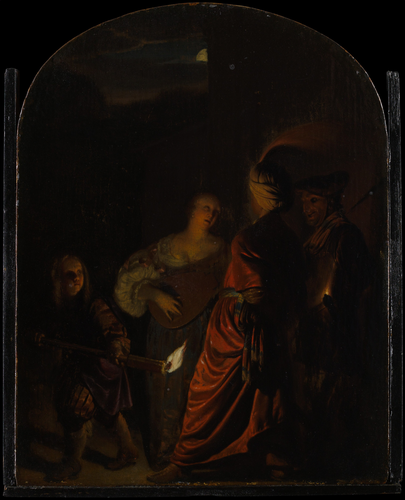
\includegraphics{paintings_files/figure-pdf/cell-2-output-14.png}

Title: The Visit

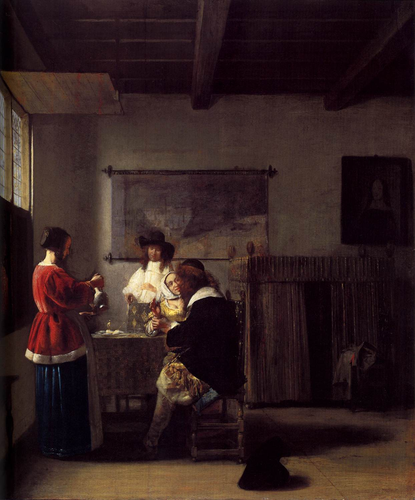
\includegraphics{paintings_files/figure-pdf/cell-2-output-16.png}

Title: Portrait of a Man Holding Gloves

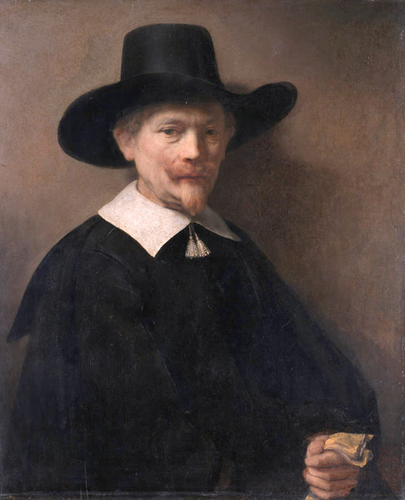
\includegraphics{paintings_files/figure-pdf/cell-2-output-18.png}

\bookmarksetup{startatroot}

\hypertarget{activity-embedded-video-in-jupyter-notebook}{%
\chapter{Activity: Embedded video in Jupyter
Notebook}\label{activity-embedded-video-in-jupyter-notebook}}

Objective: Running and editing Juypter Notebooks in MyBinder and
retrieving video and 3D models as embeds.

\hypertarget{video-embedding}{%
\section{Video embedding}\label{video-embedding}}

The below Python code experiments with retrieving video data via iframe
embedding.

\begin{verbatim}
<IPython.core.display.HTML object>
\end{verbatim}

\hypertarget{d-model-embedding}{%
\section{3D model embedding}\label{d-model-embedding}}

The below Python code experiments with retrieving 3D data via iframe
embedding.

\begin{verbatim}
<IPython.core.display.HTML object>
\end{verbatim}

\begin{verbatim}
<IPython.core.display.HTML object>
\end{verbatim}

\bookmarksetup{startatroot}

\hypertarget{custom-collection---sw}{%
\chapter{Custom Collection - SW}\label{custom-collection---sw}}

Custom Collection by Simon Worthington (April 23): Paintings by Lucas
Cranach the Elder https://www.wikidata.org/wiki/Q191748.

The collection Notebook only contains the SPARQL query and needs
additional Python adding to parse the metadata output.

Madonna under the Fir Tree
\includegraphics{sw-collection_files/figure-pdf/cell-2-output-2.png}

Saint Eustace
\includegraphics{sw-collection_files/figure-pdf/cell-2-output-4.png}

Judith with two female companions
\includegraphics{sw-collection_files/figure-pdf/cell-2-output-6.png}

Maria Hilf
\includegraphics{sw-collection_files/figure-pdf/cell-2-output-8.png}

Cupid Complaining to Venus
\includegraphics{sw-collection_files/figure-pdf/cell-2-output-10.png}

The Three Graces
\includegraphics{sw-collection_files/figure-pdf/cell-2-output-12.png}

The Crucifixion with the Converted Centurion

\begin{verbatim}
c:\Users\simon\AppData\Local\Programs\Python\Python39\lib\site-packages\PIL\Image.py:3074: DecompressionBombWarning: Image size (121328284 pixels) exceeds limit of 89478485 pixels, could be decompression bomb DOS attack.
  warnings.warn(
\end{verbatim}

\includegraphics{sw-collection_files/figure-pdf/cell-2-output-15.png}

Madonna with Child with Young John the Baptist
\includegraphics{sw-collection_files/figure-pdf/cell-2-output-17.png}

Female Portrait
\includegraphics{sw-collection_files/figure-pdf/cell-2-output-19.png}

Melancholy
\includegraphics{sw-collection_files/figure-pdf/cell-2-output-21.png}

Melancholy
\includegraphics{sw-collection_files/figure-pdf/cell-2-output-23.png}

Cardinal Albrecht of Brandenburg in front of the Crucified Christ
\includegraphics{sw-collection_files/figure-pdf/cell-2-output-25.png}

A Faun and His Family with a Slain Lion
\includegraphics{sw-collection_files/figure-pdf/cell-2-output-27.png}

Rest on the Flight to Egypt
\includegraphics{sw-collection_files/figure-pdf/cell-2-output-29.png}

The Crucifixion
\includegraphics{sw-collection_files/figure-pdf/cell-2-output-31.png}

Adam and Eve
\includegraphics{sw-collection_files/figure-pdf/cell-2-output-33.png}

Christ blessing the children.
\includegraphics{sw-collection_files/figure-pdf/cell-2-output-35.png}

Portrait of a girl with forget-me-nots
\includegraphics{sw-collection_files/figure-pdf/cell-2-output-37.png}

Herkules and Omphale
\includegraphics{sw-collection_files/figure-pdf/cell-2-output-39.png}

Madonna and Child
\includegraphics{sw-collection_files/figure-pdf/cell-2-output-41.png}

Virgin and Child with Saint Catherine of Alexandria
\includegraphics{sw-collection_files/figure-pdf/cell-2-output-43.png}

The Mystic Marriage of Saint Catherine of Alexandria with Saints
Dorothy, Margaret and Barbara
\includegraphics{sw-collection_files/figure-pdf/cell-2-output-45.png}


\backmatter

\end{document}
